\documentclass[final]{beamer}
\usepackage{multimedia}
\usepackage{color}
\usepackage[normalem]{ulem}
\graphicspath{{figures/}}

\newcommand{\comment}[1]{}
\definecolor{grigio}{rgb}{.8, .8, .8}

\mode<beamer>{%
	\usetheme{Madrid}
  \usecolortheme{beaver}
}
\titlegraphic{
\includegraphics[width=0.3\textwidth]{LogoUPF_CBC}\hspace{0.5cm}
\includegraphics[width=0.3\textwidth]{logo_italian_academy}\hspace{0.5cm}
\includegraphics[width=0.3\textwidth]{ctn_columbia}}
\title[Italian Academy]{\textbf{The topology of mental states.}\\ Combining data science and graph theory to reveal neural networks for cognitive functions.}
\author{Andrea Insabato}
\date{November 1st, 2017}

\begin{document}


\begin{frame}<handout:0>
  \titlepage
\end{frame}

\begin{frame}
\transdissolve
\frametitle{The problem}
Characterization of brain networks underlying ``mental'' states 
using data science tools
\pause
\begin{itemize}
	\item mental 
		\pause
	\item brain as a network
		\pause
	\item data science
\end{itemize}
\end{frame}

\begin{frame}
\transdissolve
\frametitle{The problem}
Example: brain network of Alzheimer desease.
\end{frame}

\begin{frame}
\frametitle{The problem: example}
\begin{center}
\includegraphics<2>[width=0.6\columnwidth]{noise_mixture7}
\includegraphics<3>[width=0.6\columnwidth]{noise_mixture6}
\includegraphics<4>[width=0.6\columnwidth]{noise_mixture5}
\includegraphics<5>[width=0.6\columnwidth]{noise_mixture4}
\includegraphics<6>[width=0.6\columnwidth]{noise_mixture3}
\includegraphics<7>[width=0.6\columnwidth]{noise_mixture2}
\includegraphics<8>[width=0.6\columnwidth]{noise_mixture1}
\includegraphics<9>[width=0.6\columnwidth]{noise_mixture0}
\end{center}
\end{frame}

\begin{frame}
\transdissolve
\frametitle{The problem and subproblems}
\begin{itemize}
	\item Characterization of brain networks underlying ``mental'' states 
using data science tools
\pause
	\item Separate different sources of varibility/noise
\pause
	\begin{itemize}
		\item classify individuals
			\pause
		\item classify conditions 
			\pause
		\item extract networks underlying each classification
	\end{itemize}
\end{itemize}
\end{frame}

\begin{frame}
\frametitle{Data}
\begin{itemize}
	\item fMRI
	\item BOLD signal
\end{itemize}
\begin{center}
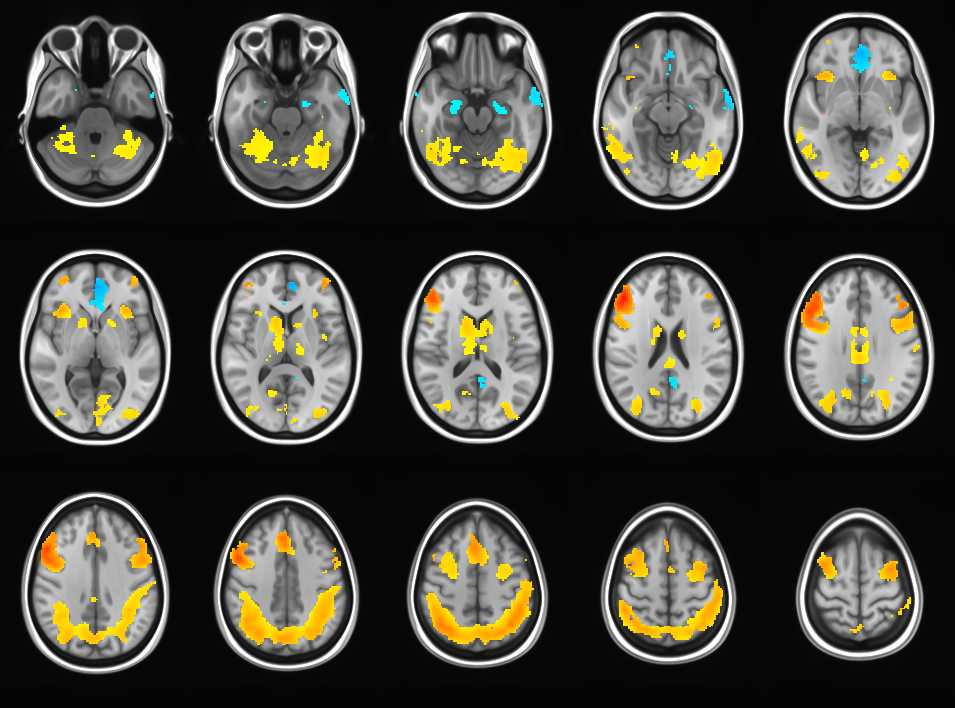
\includegraphics[width=0.7\columnwidth]{fmri}
\end{center}

\end{frame}

\begin{frame}
\frametitle{Data}
\begin{center}
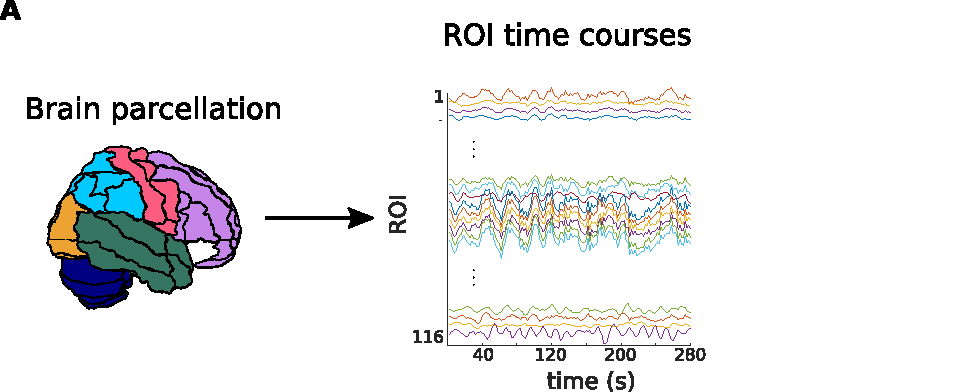
\includegraphics[width=0.8\columnwidth]{fig1b}
\end{center}
\end{frame}

\begin{frame}
\frametitle{Statistical association: correlation}
\begin{center}
\includegraphics<1>[width=0.9\columnwidth]{correlation}
\includegraphics<2>[width=0.5\columnwidth]{toy_FC}
\includegraphics<3>[width=0.8\columnwidth]{correlation_xkcd}
\end{center}
\end{frame}

\begin{frame}
\frametitle{FC}
\begin{center}
\includegraphics<1>[width=0.8\columnwidth]{fig1b}
\includegraphics<2>[width=0.8\columnwidth]{fig1a}
\end{center}
\end{frame}

\begin{frame}
\frametitle{EC}
\begin{center}
\includegraphics<1>[width=0.6\columnwidth]{model}
\transdissolve
\includegraphics<2>[width=0.65\columnwidth]{fitting}
\end{center}
\end{frame}

\begin{frame}
\frametitle{Subjects classification: EC as fingerprint}
\begin{center}
\includegraphics<1>[width=0.7\columnwidth]{fingerprint}
\transdissolve
\includegraphics<2>[width=0.65\columnwidth]{pipeline}
\end{center}
\end{frame}

\begin{frame}
\transdissolve
\frametitle{The problem and subproblems}
\begin{itemize}
	\item Characterization of brain networks underlying ``mental'' states 
using data science tools
	\begin{itemize}
		\item \alert<2->{classify individuals}
		\item \color<2>{grigio}{classify conditions} 
		\item \color<2>{grigio}{extract networks underlying each classification}
	\end{itemize}
\end{itemize}
\end{frame}

\begin{frame}
\frametitle{Subjects classification}
\begin{center}
\includegraphics<1>[width=0.9\columnwidth]{class_subj}
\end{center}
\end{frame}

\begin{frame}
\frametitle{The classifier}
\begin{center}
\includegraphics<2>[width=0.6\columnwidth]{regression3}
\includegraphics<3>[width=0.6\columnwidth]{regression2}
\includegraphics<4>[width=0.6\columnwidth]{regression1}
\includegraphics<5>[width=0.6\columnwidth]{regression0}
\includegraphics<6>[width=0.6\columnwidth]{regression-1}
\includegraphics<7>[width=0.6\columnwidth]{regression4}
\end{center}
\end{frame}

\begin{frame}
\frametitle{Subjects network}
\begin{center}
\includegraphics<1>[width=0.8\columnwidth]{subj_varying_links}
\end{center}
\end{frame}

\begin{frame}
\frametitle{Subjects network}
\begin{center}
\includegraphics<1>[width=0.8\columnwidth]{subj_net}
\end{center}
\end{frame}

\begin{frame}
\frametitle{Agreement between datasets}
\begin{center}
\includegraphics<1>[width=0.9\columnwidth]{avg_ranking_subsystems}
\end{center}
\end{frame}

\begin{frame}
\frametitle{Agreement between datasets}
\begin{center}
\includegraphics<1>[width=0.6\columnwidth]{subj_H0}
\end{center}
\end{frame}

\begin{frame}
\transdissolve
\frametitle{The problem and subproblems}
\begin{itemize}
	\item Characterization of brain networks underlying ``mental'' states 
using data science tools
	\begin{itemize}
		\item \color<2>{grigio}{classify individuals}
		\item \alert<2>{classify conditions} 
		\item \color<2>{grigio}{extract networks underlying each classification}
	\end{itemize}
\end{itemize}
\end{frame}

\begin{frame}
\frametitle{Simultaneous classification: subjects and conditions}
\begin{center}
\includegraphics[width=0.6\columnwidth]{noise_mixture0}
\end{center}
\end{frame}

\begin{frame}
\frametitle{Simultaneous classification: subjects and conditions}
\begin{center}
\includegraphics<1>[width=0.6\columnwidth]{subj_cond_idea}
\end{center}
\end{frame}

\begin{frame}
\frametitle{Simultaneous classification: subjects and conditions}
\begin{center}
\includegraphics<1>[width=0.6\columnwidth]{subj_cond_results}
\end{center}
\end{frame}

\begin{frame}
\frametitle{Simultaneous classification: subjects and conditions}
\begin{center}
\includegraphics<1>[width=0.6\columnwidth]{subj_cond_matrix}
\end{center}
\end{frame}

\begin{frame}
\frametitle{Simultaneous classification: subjects and conditions}
\begin{center}
\includegraphics<1>[width=0.6\columnwidth]{cond_H0}
\end{center}
\end{frame}

\begin{frame}
\frametitle{Simultaneous classification: subjects and conditions}
\begin{center}
\includegraphics<1>[width=0.7\columnwidth]{fig5}
\end{center}
\end{frame}

\begin{frame}
\frametitle{Summary}
\begin{itemize}
	\item Characterization of brain networks underlying ``mental'' states 
using data science tools
	\begin{itemize}
		\item {\color<2->{green}classify individuals}
		\item {\color<3->{green}classify conditions}
		\item \color<4->{green}extract networks underlying each classification
	\end{itemize}
\item \uncover<5->{Refinements: small samples \uncover<6>{$\rightarrow$ Bayesian inference}}
\end{itemize}
\end{frame}

\begin{frame}
\frametitle{Acknowledgments}
\begin{columns}
\begin{column}{0.5\textwidth}
\begin{center}
	\alert<2>{Vicente Pallares}\\
\vspace{1cm}

\alert<2>{Matthieu Gilson}\\
\vspace{1cm}

\small Ana Sanjuan\\
\vspace{0.5cm}

\small Simone Kuhn\\
\vspace{0.5cm}

\small Dante Mantini\\
\vspace{0.5cm}

\small Gustavo Deco\\
\end{center}
\end{column}
\begin{column}{0.5\textwidth}
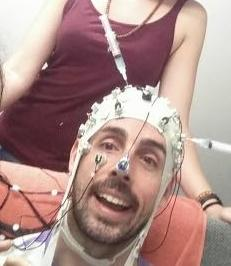
\includegraphics[width=0.5\columnwidth,valign=t]{vicente2}
\vspace{0.5cm}

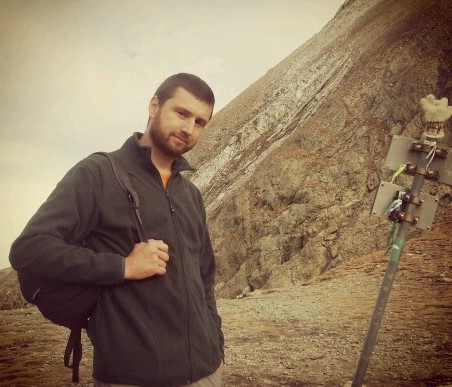
\includegraphics[width=0.5\columnwidth,valign=t]{matt}
\end{column}
\end{columns}
\end{frame}

\begin{frame}
\frametitle{}
\begin{center}
\includegraphics<1>[width=0.6\columnwidth]{minion}
\end{center}
\end{frame}



\end{document}
